\section{Технический проект}


\subsection{Общая характеристика организации решения задачи}
Необходимо спроектировать и разработать программно-информационную систему, которая способствует оптимизации ресторанного бизнеса.  
Программа представляет собой набор модулей, которые помогут оптимизировать и автоматизировать такие процессы, как управление заказами и персоналом, учет ресурсов, формирование отчетности.
Программа написана на языке программирования Python.


\subsection{Обоснование выбора технологии проектирования}
На сегодняшний день информационный рынок, поставляющий программные решения в выбранной сфере, предлагает множество продуктов, позволяющих достигнуть поставленной цели – разработки приложения.


\subsubsection{Описание используемых технологий и языков программирования}
В процессе разработки программного продукта был использован язык программирования Python, его объекты и библиотеки, а также объектно-реляционная система управления базами данных PostgreSQL.


\subsubsection{Язык программирования Python}
Python — высокоуровневый язык программирования. Он широко используется во всем мире для самых разных целей — базы данных и обработка текстов, встраивание интерпретатора в игры, программирование GUI и быстрое создание прототипов (RAD)\cite{python}.

\paragraph{Библиотека Tkiner}
Tkinter — это модуль Python, который работает с библиотекой Tk - стандартной библиотекой Python \cite{tkiner}. С помощью данной библиотеки было реализовано множество проектов, благодаря ее доступности, универсальности и эффективности. Библиотека представляет собой набор виджетов, например, кнопки, метки, текстовые поля. Не менее важным является тот факт, что tkiner поддерживает кроссплатформенность, что позволяет, приложениям работать на различных операционных системах.

\subsubsection{PostgerSQL} 


PostgreSQL, или просто postgres, –  мощная объектно-реляционная СУБД с открытым исходным кодом, которая позволяет создавать высоконагруженные базы данных большого объема \cite{postgrestermin}. Преимуществами данной системы является её расширяемость, техническое совершенство и совместимость. Используют postgreSQL в различных сферах, начиная от коммерческих продуктов и заканчивая госучреждениями. Плюсом posgres является её кросс-платформленность, что позволяет использовать готовый продукт в большинстве современных операционных систем.


\paragraph{Достоинства PostgerSQL}
С точки зрения пользователя PosqreSQL обладает следующими преимуществами:
\begin{itemize}
 	\item регулярный обновления;
 	\item общирная документация;
 	\item широкий арсенал расширений;
 	\item бесплатный исходный код;
 	\item возможность автоматизированного решения администраторских задач;
 	\item интеграция с другими СУБД \cite{postgres}.
\end{itemize}
PosgreSQL также будет хорошим выбором и с точки зрения бизнеса:
\begin{itemize}
	\item бесплатная лицензия;
	\item система хорошо масштабируется;
	\item posqres обеспечивает высокую производительность;
	\item не имеет ограничений на количество развернутых экземпляров;
	\item является кросс-платформленным ПО;
	\item обладает высокой надежностью.
\end{itemize}	
	


\subsection{Диаграмма компонентов и схема обмена данными между файлами компонента}

Диаграмма компонентов — это, фактически, список артефактов, из которых состоит моделируемая система, с указанием некоторых отношений между артефактами \cite{components}.
В данной диаграмме компонентом считается как программные составляющие, например, база данных и пользовательский интерфейс, так и аппаратные - схема, устройство. На рисунке  ~\ref{componetdiag:image} представлена диаграмма компонентов для проектируемой системы. На данной диаграмме изображён сервер, база данных, кассовый терминал и модули системы.
\begin{figure}[ht]
\centering
\includegraphics[width=1\linewidth]{componetdiag}
\caption{Диаграмма компонентов}
\label{componetdiag:image}
\end{figure}


\subsection{Структура базы данных}
Сущности и отношение между таблицами базы данных отражены на рисунке~\ref{erd:image}.
\begin{figure}[ht]
	\centering
	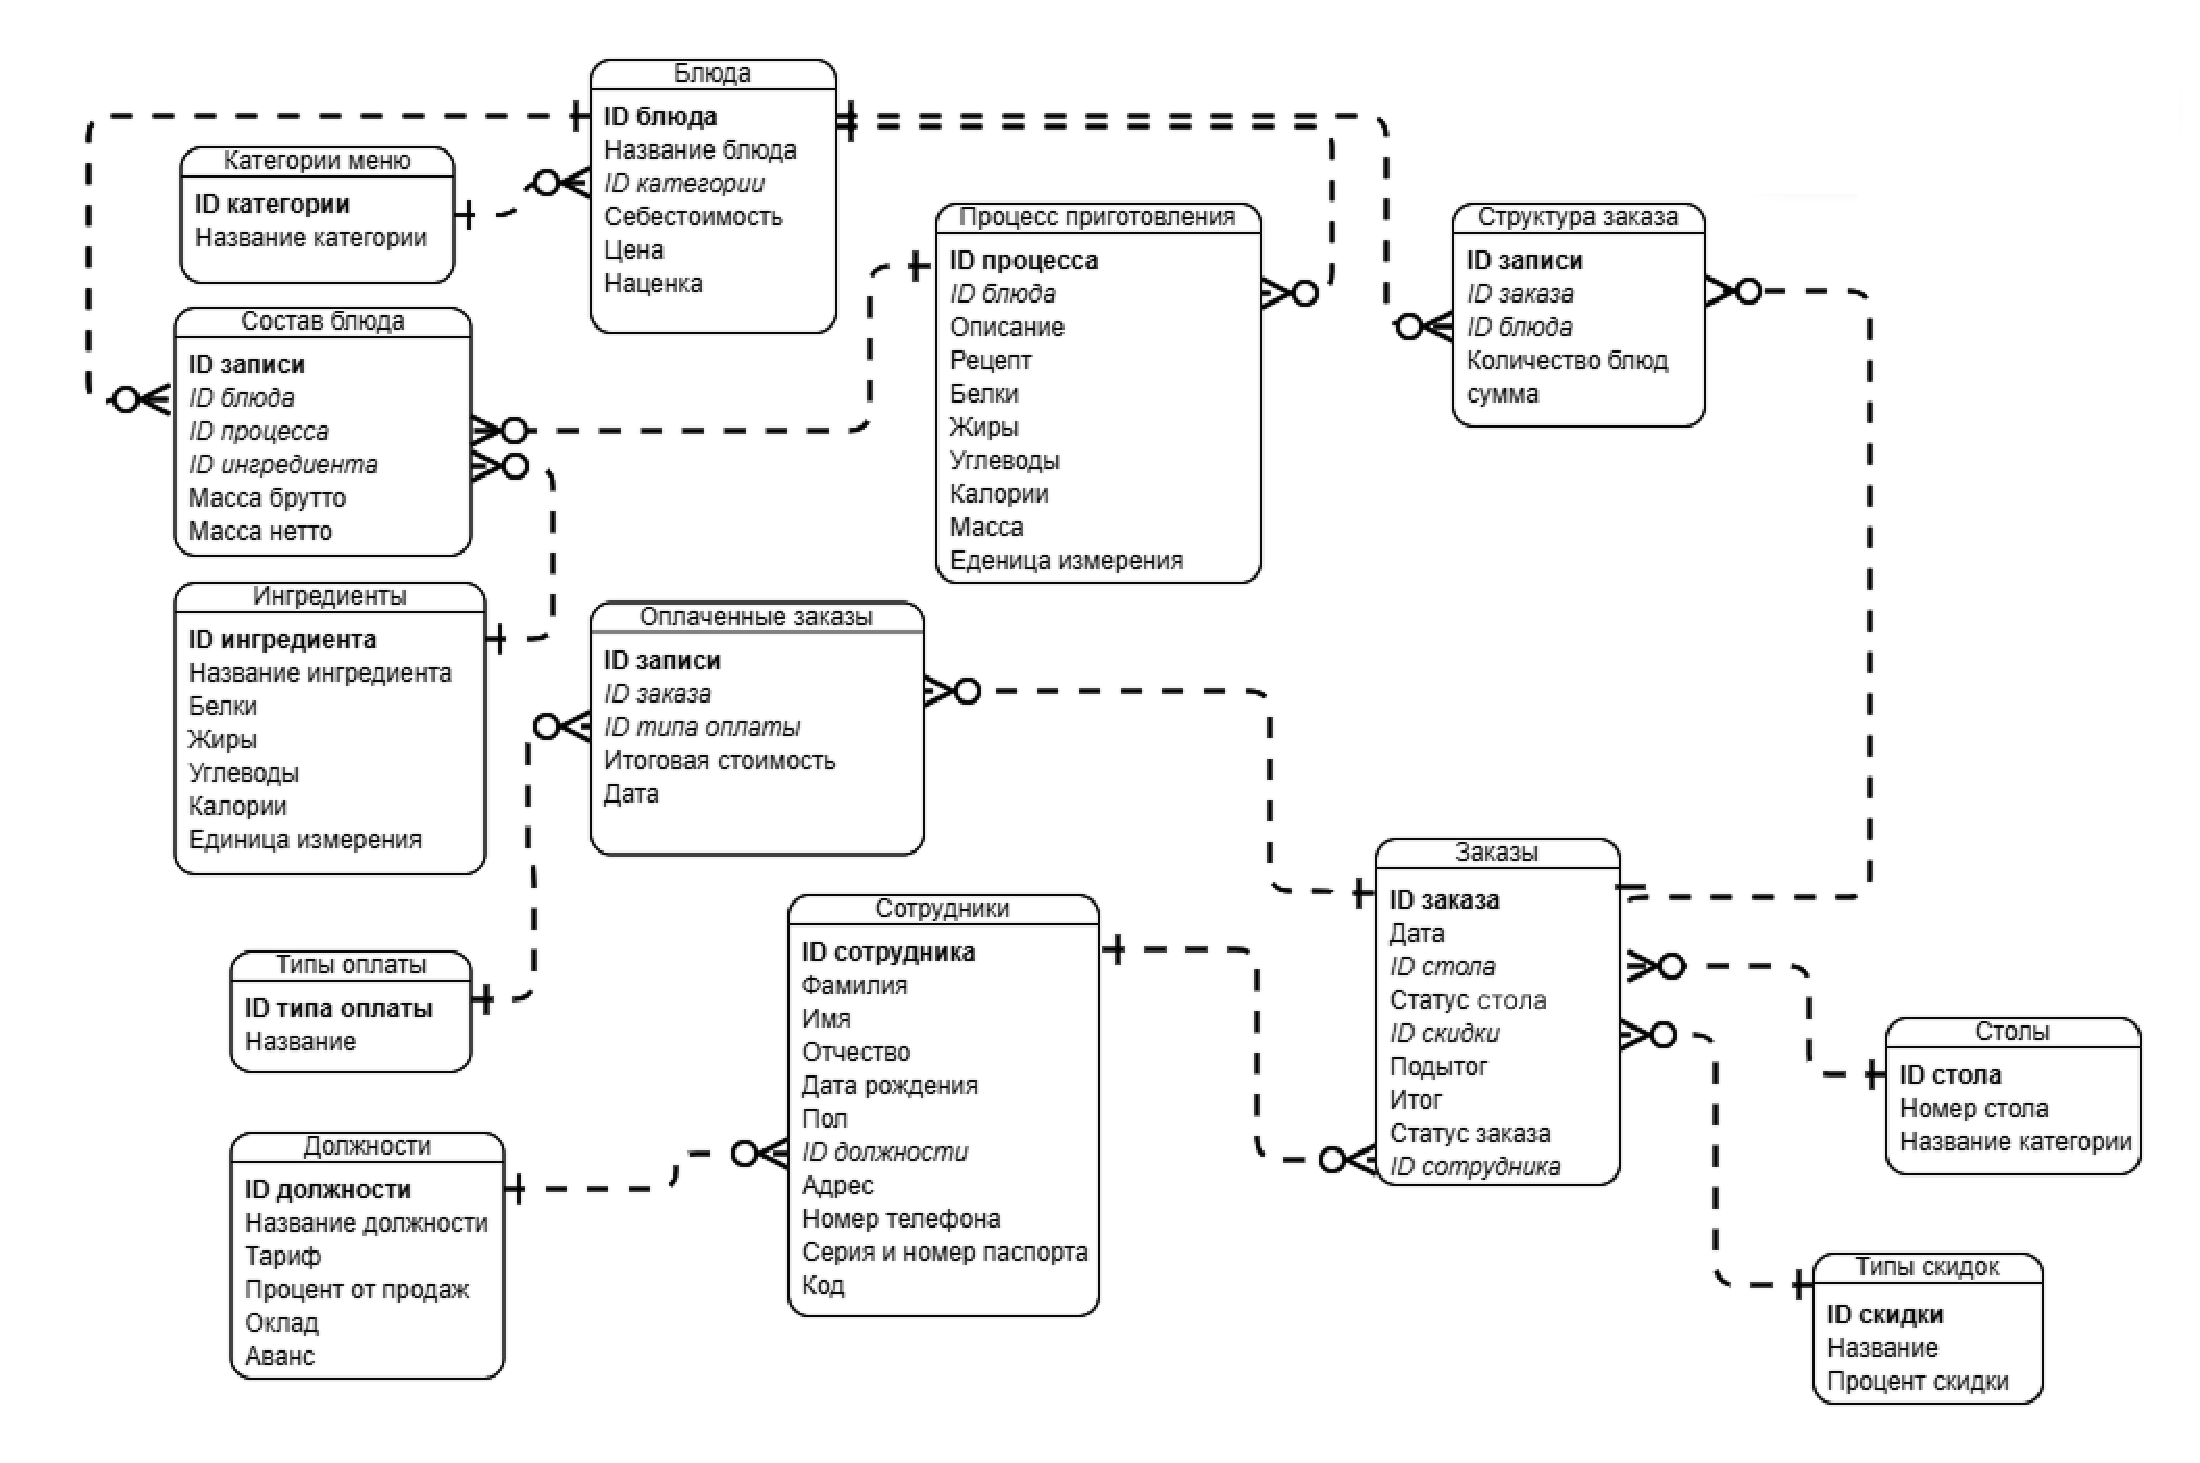
\includegraphics[width=1\linewidth]{erd}
	\caption{ER-диаграмма}
	\label{erd:image}
\end{figure}
\newline
В таблице \ref{staff:table} представлена структура таблицы staff.
\begin{xltabular}{\textwidth}{|l|p{4.5cm}|p{2.2cm}|X|}
	\caption{Таблица staff\label{staff:table}}\\ \hline
	\centrow  Тип ключа & \centrow Имя столбца & \centrow  Тип данных & \centrow Обязательность \\ \hline
	\endfirsthead
	\continuecaption{Продолжение таблицы \ref{staff:table}} 
	\centrow  Тип ключа & \centrow Имя столбца & \centrow  Тип данных & \centrow Обязательность   \\ \hline
	\finishhead
	primary key & id\_staff & Integer & true  \\ \hline 
	~ & last\_name & Text & true  \\ \hline 
	~ & first\_name & Text & true  \\ \hline 
	~ & middle\_name & Text & false \\ \hline
	~ & birth & Date & true  \\ \hline 
	~ & gender & Text & true  \\ \hline 
	foreing key & id\_post & Integer & true \\ \hline 
	~ & adress & Text & false\\ \hline 
	~ & phone\_number & Bigint & true  \\ \hline
	~ & ser\_num\_pass & Bigint & false \\ \hline
	~ & code & Integer & true
\end{xltabular}


В таблице \ref{post:table} представлена структура таблицы post.
\begin{xltabular}{\textwidth}{|l|p{4.5cm}|p{2.2cm}|X|}
	\caption{Таблица post\label{post:table}}\\ \hline
	\centrow  Тип ключа & \centrow Имя столбца & \centrow  Тип данных & \centrow Обязательность \\ \hline
	\endfirsthead
	\continuecaption{Продолжение таблицы \ref{post:table}} 
	\centrow  Тип ключа & \centrow Имя столбца & \centrow  Тип данных & \centrow Обязательность   \\ \hline
	\finishhead
	primary key & id\_post & Integer & true \\ \hline 
	~ & name\_post & Text & true  \\ \hline 
	~ & rate & Numeric & true  \\ \hline 
	~ & percent & Text & false  \\ \hline
	~ & selary & Date & false\\ \hline 
	~ & advance & Text & false    
\end{xltabular}

В таблице \ref{order:table} представлена структура таблицы order.
\begin{xltabular}{\textwidth}{|l|p{4.5cm}|p{2.2cm}|X|}
	\caption{Таблица order\label{order:table}}\\ \hline
	\centrow  Тип ключа & \centrow Имя столбца & \centrow  Тип данных & \centrow Обязательность \\ \hline
	\endfirsthead
	\continuecaption{Продолжение таблицы \ref{order:table}} 
	\centrow  Тип ключа & \centrow Имя столбца & \centrow  Тип данных & \centrow Обязательность   \\ \hline
	\finishhead
	primary key & id\_order & Integer & true \\ \hline 
	~ & date & Date & true \\ \hline 
	foreing key & id\_table & Text & true \\ \hline 
	~ & status\_ordere & Integer & true  \\ \hline
	foreing key & id\_sale & Text & true  \\ \hline 
	~ & summary & Numeric & true \\ \hline 
	~ & result & Integer & true \\ \hline 
	~ & order\_condition & Text & false
\end{xltabular}

В таблице \ref{tables:table} представлена структура таблицы tables.
\begin{xltabular}{\textwidth}{|l|p{4.5cm}|p{2.2cm}|X|}
	\caption{Таблица tables\label{tables:table}}\\ \hline
	\centrow  Тип ключа & \centrow Имя столбца & \centrow  Тип данных & \centrow Обязательность \\ \hline
	\endfirsthead
	\continuecaption{Продолжение таблицы \ref{tables:table}} 
	\centrow  Тип ключа & \centrow Имя столбца & \centrow  Тип данных & \centrow Обязательность   \\ \hline
	\finishhead
	primary key & id\_tabel & Integer & true \\ \hline 
	~ & number\_tabel & Integer & true \\ \hline 
	~ & name\_tabel & Text & true 
\end{xltabular}

В таблице \ref{paytype:table} представлена структура таблицы pay\_types.
\begin{xltabular}{\textwidth}{|l|p{4.5cm}|p{2.2cm}|X|}
	\caption{Таблица pay\_types\label{paytype:table}}\\ \hline
	\centrow  Тип ключа & \centrow Имя столбца & \centrow  Тип данных & \centrow Обязательность \\ \hline
	\endfirsthead
	\continuecaption{Продолжение таблицы \ref{paytype:table}} 
	\centrow  Тип ключа & \centrow Имя столбца & \centrow  Тип данных & \centrow Обязательность   \\ \hline
	\finishhead
	primary key & id\_type & Integer & true \\ \hline 
	~ & name\_type & Text & true 
\end{xltabular}

В таблице \ref{structureorder:table} представлена структура таблицы structure\_order.
\begin{xltabular}{\textwidth}{|l|p{4.5cm}|p{2.2cm}|X|}
	\caption{Таблица structure\_order\label{structureorder:table}}\\ \hline
	\centrow  Тип ключа & \centrow Имя столбца & \centrow  Тип данных & \centrow Обязательность \\ \hline
	\endfirsthead
	\continuecaption{Продолжение таблицы \ref{structureorder:table}} 
	\centrow  Тип ключа & \centrow Имя столбца & \centrow  Тип данных & \centrow Обязательность   \\ \hline
	\finishhead
	primary key & id\_record & Integer & true \\ \hline 
	foreing key & id\_order & Integer & true \\ \hline 
	foreing key & id\_dish & Integer & true \\ \hline 
	~ & status\_ordere & Integer & true  \\ \hline 
	~ & dish\_quantity & Integer & true \\ \hline 
	~ & sum & Numeric & true  
\end{xltabular}

В таблице \ref{paidorders:table} представлена структура таблицы paid\_orders.
\begin{xltabular}{\textwidth}{|l|p{4.5cm}|p{2.2cm}|X|}
	\caption{Таблица paid\_orders\label{paidorders:table}}\\ \hline
	\centrow  Тип ключа & \centrow Имя столбца & \centrow  Тип данных & \centrow Обязательность \\ \hline
	\endfirsthead
	\continuecaption{Продолжение таблицы \ref{paidorders:table}} 
	\centrow  Тип ключа & \centrow Имя столбца & \centrow  Тип данных & \centrow Обязательность   \\ \hline
	\finishhead
	primary key & id\_data & Integer & true \\ \hline 
	foreing key & id\_order & Integer & true \\ \hline 
	foreing key & id\_pay\_type & Text & true \\ \hline 
	~ & sum & Integer & true  \\ \hline
	~ & date & Text & true  \\ \hline 
	~ & summary & Numeric & true \\ \hline 
	~ & result & Integer & true \\ \hline 
	~ & order\_condition & Text & true
\end{xltabular}

В таблице \ref{paytypes:table} представлена структура таблицы pay\_types.
\begin{xltabular}{\textwidth}{|l|p{4.5cm}|p{2.2cm}|X|}
	\caption{Таблица pay\_types\label{paytypes:table}}\\ \hline
	\centrow  Тип ключа & \centrow Имя столбца & \centrow  Тип данных & \centrow Обязательность \\ \hline
	\endfirsthead
	\continuecaption{Продолжение таблицы \ref{paytypes:table}} 
	\centrow  Тип ключа & \centrow Имя столбца & \centrow  Тип данных & \centrow Обязательность   \\ \hline
	\finishhead
	primary key & id\_type & Integer & true \\ \hline 
	~ & name\_type & Text & true
\end{xltabular}

В таблице \ref{menudishprocess:table} представлена структура таблицы menu\_dish\_process.
\begin{xltabular}{\textwidth}{|l|p{4.5cm}|p{2.2cm}|X|}
	\caption{Таблица menu\_dish\_process\label{menudishprocess:table}}\\ \hline
	\centrow  Тип ключа & \centrow Имя столбца & \centrow  Тип данных & \centrow Обязательность \\ \hline
	\endfirsthead
	\continuecaption{Продолжение таблицы \ref{menudishprocess:table}} 
	\centrow  Тип ключа & \centrow Имя столбца & \centrow  Тип данных & \centrow Обязательность   \\ \hline
	\finishhead
	primary key & id\_process & Integer & true  \\ \hline 
	foreing key & id\_dish & Integer & true  \\ \hline 
	~ & description & Text & true  \\ \hline 
	~ & recept & Text & false \\ \hline
	~ & birth & Date & false  \\ \hline 
	~ & proteins & Numeric & false  \\ \hline 
	~ & fats & Numeric & false \\ \hline 
	~ & carbohydrates & Numeric & false\\ \hline 
	~ & calories & Numeric & false  \\ \hline
	~ & massa & Numeric & false \\ \hline
	~ & ed\_ismereni & Text & false
\end{xltabular}

В таблице \ref{dish:table} представлена структура таблицы menu\_dishes.
\begin{xltabular}{\textwidth}{|l|p{4.5cm}|p{2.2cm}|X|}
	\caption{Таблица menu\_dishes\label{dish:table}}\\ \hline
	\centrow  Тип ключа & \centrow Имя столбца & \centrow  Тип данных & \centrow Обязательность \\ \hline
	\endfirsthead
	\continuecaption{Продолжение таблицы \ref{dish:table}} 
	\centrow  Тип ключа & \centrow Имя столбца & \centrow  Тип данных & \centrow Обязательность   \\ \hline
	\finishhead
	primary key & id\_dish & Integer & true \\ \hline 
	~ & name\_dish & Text & true  \\ \hline
	foreing key  & id\_category & Integer & true  \\ \hline 
	~ & cost\_dish & Numeric & true \\ \hline
	~ & price\_dish & Numeric & true  \\ \hline 
	~ & extra\_dish & Numeric & true 
\end{xltabular}

В таблице \ref{category:table} представлена структура таблицы menu\_category.
\begin{xltabular}{\textwidth}{|l|p{4.5cm}|p{2.2cm}|X|}
	\caption{Таблица pay\_types\label{category:table}}\\ \hline
	\centrow  Тип ключа & \centrow Имя столбца & \centrow  Тип данных & \centrow Обязательность \\ \hline
	\endfirsthead
	\continuecaption{Продолжение таблицы \ref{category:table}} 
	\centrow  Тип ключа & \centrow Имя столбца & \centrow  Тип данных & \centrow Обязательность   \\ \hline
	\finishhead
	primary key & id\_category & Integer & true \\ \hline 
	~ & name\_category & Text & true
\end{xltabular}

В таблице \ref{composition:table} представлена структура таблицы menu\_dish\_composition.
\begin{xltabular}{\textwidth}{|l|p{4.5cm}|p{2.2cm}|X|}
	\caption{Таблица menu\_dish\_composition\label{composition:table}}\\ \hline
	\centrow  Тип ключа & \centrow Имя столбца & \centrow  Тип данных & \centrow Обязательность \\ \hline
	\endfirsthead
	\continuecaption{Продолжение таблицы \ref{composition:table}} 
	\centrow  Тип ключа & \centrow Имя столбца & \centrow  Тип данных & \centrow Обязательность   \\ \hline
	\finishhead
	primary key & id\_composition & Integer & true  \\ \hline 
	foreing key & id\_dish & Integer & true  \\ \hline 
	foreing key & id\_process & Integer & true  \\ \hline 
	foreing key & id\_ingredient & Integer & true  \\ \hline 
	~ & massa\_brytto & Numeric & true  \\ \hline 
	~ & massa\_netto & Numeric & true 
\end{xltabular}

В таблице \ref{ingredients:table} представлена структура таблицы menu\_ingredient.
\begin{xltabular}{\textwidth}{|l|p{4.5cm}|p{2.2cm}|X|}
	\caption{Таблица menu\_ingredient\label{ingredients:table}}\\ \hline
	\centrow  Тип ключа & \centrow Имя столбца & \centrow  Тип данных & \centrow Обязательность \\ \hline
	\endfirsthead
	\continuecaption{Продолжение таблицы \ref{ingredients:table}} 
	\centrow  Тип ключа & \centrow Имя столбца & \centrow  Тип данных & \centrow Обязательность   \\ \hline
	\finishhead
	primary key & id\_ingredient & Integer & true  \\ \hline 
	~ & name\_ingredient & Text & true  \\ \hline
	~ & proteins & Numeric & false  \\ \hline 
	~ & fats & Numeric & false \\ \hline 
	~ & carbohydrates & Numeric & false\\ \hline 
	~ & calories & Numeric & false  \\ \hline
	~ & massa & Numeric & false \\ \hline
	~ & ed\_ismereni & Text & false
\end{xltabular}


